\documentclass[letterpaper, 10 pt, conference]{ieeeconf}  
\IEEEoverridecommandlockouts                              
\overrideIEEEmargins

\usepackage[utf8]{inputenc}
\usepackage[T1]{fontenc}
\usepackage{graphicx}
\usepackage{float}
\usepackage{comment}
\usepackage{hyperref}
\PassOptionsToPackage{hyphens}{url}
\usepackage{listings}
\usepackage{xcolor}
\usepackage{etoolbox}    

\definecolor{codegreen}{rgb}{0,0.6,0}
\definecolor{codegray}{rgb}{0.5,0.5,0.5}
\definecolor{codepurple}{rgb}{0.58,0,0.82}
\definecolor{backcolour}{rgb}{0.95,0.95,0.92}

\lstdefinestyle{mystyle}{
    backgroundcolor=\color{backcolour},   
    commentstyle=\color{codegreen},
    keywordstyle=\color{magenta},
    numberstyle=\tiny\color{codegray},
    stringstyle=\color{codepurple},
    basicstyle=\ttfamily\footnotesize,
    breakatwhitespace=false,         
    breaklines=true,                 
    captionpos=b,                     
    numbers=left,                    
    numbersep=5pt,                  
    showspaces=false,                
    showstringspaces=false,
    showtabs=false,       
    stepnumber=1,
    frame=none,                    
    %columns=fullflexible,
    keepspaces=true,
    %xleftmargin=\parindent,
    tabsize=4
}

\lstdefinestyle{consolestyle}{
    backgroundcolor=\color{backcolour},   
    commentstyle=\color{codegreen},
    keywordstyle=\color{magenta},
    numberstyle=\tiny\color{codegray},
    stringstyle=\color{codepurple},
    basicstyle=\ttfamily\footnotesize,
    breaklines=true,  
}

\title{\LARGE \bf
Didactic application of an f-OFDM transceiver in Mathworks Simulink}

\author{Levy G. da S. Galvão$^{1}$ e Luiz G. de Q. S. Júnior$^{2}$% <-this % stops a space
\thanks{*This work was not supported by any organization}% <-this % stops a space
\thanks{$^{1}$ Electrical engineering undergraduate, Universidade Federal do Rio Grande do Norte, Brazil.}%
\thanks{$^{2}$ Telecommunications engineering Ph.D, Universidade Federal do Rio Grande do Norte, Brazil.}%
}

\begin{document}

\maketitle
\thispagestyle{empty}
\pagestyle{empty}

\begin{abstract}
Com o objetivo \url{http://www.leca.ufrn.br/~pmotta}.\url{pmotta@leca.ufrn.br}. \lipsum[1]
\end{abstract}
\textbf{Palavras-chaves}: palavras. chaves.
\pagebreak
\tableofcontents
\pagebreak
\section{INTRODUCTION}

Orthogonal Frequency Division Multiplexing (OFDM) has become a key modulation scheme in modern wireless communications e.g. some radio interfaces of wireless LAN (WLAN), 4G Long-Term Evolution (LTE), terrestrial digital and mobile TV systems, and lately, a powerful candidate for 5G.

The OFDM combines multiples M-QAM symbols transmitted at the same time span but separated in frequency, with each M-QAM symbol been modulated by a different carrier. This results in a larger symbol period, that is more robust to intersymbol interference (ISI).

The main aspect that differs OFDM from Frequency Division Multiplexing (FDM) is that OFDM does not need a high guard band between subchannels, since its subcarriers obey the principle of orthogonality and they can be closely separated and even partially overlapping. This feature causes a natural efficient use of the available spectrum and reliability to intercarrier interference (ICI).

Despite OFDM advantages it can not meet the heterogeneous criteria that 5G demands, because its high side lobes in frequency once its spectrum decays slowly out of the pass band, also a large peak-to-average power ratio (PAPR) and only supports one kind of waveform in the whole bandwidth \cite{abdoli2015filtered, cheng2016filtered}. 

The solution is to implement a new kind of OFDM that retain its advantages and overcome the drawbacks, which is named filtered-OFDM (f-OFDM). The f-OFDM consists in a subband-based splitting and filtering by different filters to shape different waveforms to attend diverse application scenarios \cite{cheng2016filtered, zhang2015filtered, zhang2017filtered}.

Therefore this work implements a f-OFDM transceiver in Mathwork Simulink based in the approach of \cite{cheng2016filtered}, whose use FIR filters designed by the window function method. The remaining theoretical basis relies on the studies of \cite{ abdoli2015filtered, zhang2015filtered, zhang2017filtered, de2019comparing, al2020improving} whose supports the development of f-OFDM technology.

This paper will be divided in the following parts:

\begin{itemize}
    \item Design of an OFDM transceiver in Mathworks Simulink;
    \item Design of a FIR filter by the window function method;
    \item Incorporate the FIR filter to transform the OFDM transceiver in an f-OFDM transceiver;
    \item Check the resulting waveforms and compare them;
    \item Make final comments on the results.
\end{itemize}
\section{DEVELOPMENT}

\subsection{OFDM transceiver}

The conception of this transceiver is based on the Software Defined Radio (SDR) Experiments proposed at \cite{ece489}.

This transceiver will use a M-QAM modulator/demodulator with 16 levels, i.e. a 16-QAM ($M=16$). The number of data subcarriers was set to 48 ($N=48$), therefore each frame will contain $N\times log_2(M) = 192$ bits. The cyclic prefix has a length of 16 samples ($C=16$).

\subsubsection{Generate information bits}

The information bits are generated randomly with the block \textbf{Bernoulli binary generator} of figure \ref{fig:block1}. Its principal parameters was configured as follows:

\begin{itemize}
    \item The \textbf{probability of a zero} to be generated was set to 50\%, meaning a equal probability to generate 0's and 1's. This feature could be very important in more complex studies that deal with detection and estimation, but for the sake of simplicity this work will not take this parameter as important; 
    \item The output of this block is \textbf{frame-based} and value of type \textbf{boolean}, with each \textbf{frame of size} $F_r = N\times log_2(M) = 192$ bits.
    \item The \textbf{sample time} depends on the frame size $F_r$ and it was choose to obey a bit rate of $192 kbps$, so a sample time of $1/(192\times 10^3)$ seconds.
\end{itemize}

\begin{figure}[h]
\begin{center}
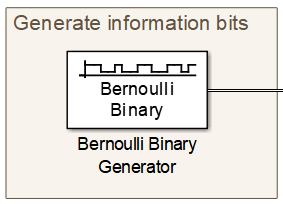
\includegraphics[width=4cm]{images/block1.png}
\caption{Bernoulli Binary Generator which marks the begin of the transmission chain and its output it is connected to the M-QAM modulator. Source: own.}
\label{fig:block1} 
\end{center}
\end{figure}

\subsubsection{Map frame bits into a M-QAM constellation}

This section uses a \textbf{rectangular QAM modulator in baseband} to map the incoming frame bits as in ifgure \ref{fig:block2}. It takes boolean balues as input (bit) and it is configured to a \textbf{16-QAM} of $M=16$, so a following gain block to \textbf{normalize} the output should divide modulator output by $\sqrt{M} = \sqrt{16}$. 

In terms of the output dimensions, the 16-QAM modulator takes a frame of 192 bits and map each set of 4 bits into a constellation point, so it outputs a total of 48 symbols of which represent the $N=48$ data subcarriers.

\begin{figure}[h]
\begin{center}
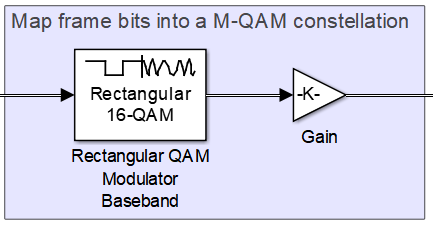
\includegraphics[width=5cm]{images/block2.png}
\caption{Rectangular QAM Modulator in baseband followed by a negative gain of which outputs to the OFDM transmitter. Source: own.}
\label{fig:block2} 
\end{center}
\end{figure}

\subsubsection{OFDM transmitter}

This block is the most complex of this system and its higher layer is represented by a Simulink subsystem as in figure \ref{fig:block3}. This section will detail each section of this subsystem.

\begin{figure}[h]
\begin{center}
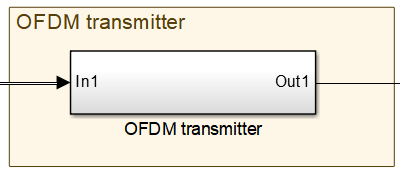
\includegraphics[width=5cm]{images/block3.png}
\caption{Higher layer from the OFDM transmitter which receive the M-QAM symbols and turn them into OFDM symbols and outputs to the AWGN channel. Source: own.}
\label{fig:block3} 
\end{center}
\end{figure}

The OFDM transmitter architecture is based in the receiving of 48 M-QAM symbols, with each symbol modulating a subcarrier; the insertion of 11 guard bands; the insertion of 1 DC subcarrier; the insertion of 4 pilot subcarriers by pilot signals with fixed values, trying to mimic a known synchronization word to facilitate coherent detection (since synchronization it is not the objective of this work, the pilot signals are arbitrary). The combination of these 64 combined subcarriers demands a IFFT of length 64. Further there is a cyclic prefix of length $C=16$ samples.

The first block to deal with the input is a \textbf{multiport selector}. It is used to address the 48 16-QAM symbols in a particular sequence that allows the alternation of data symbols, pilot symbols and the DC subcarrier. This selector has 6 outputs, with each port giving out a sequence of symbols so:

\begin{itemize}
    \item Port 1: symbols 1 to 5;
    \item Port 2: symbols 6 to 18;
    \item Port 3: symbols 19 to 24;
    \item Port 4: symbols 25 to 30;
    \item Port 5: symbols 31 to 43;
    \item Port 6: symbols 44 to 48;    
\end{itemize}

Each port connects with a respective port in a block of \textbf{matrix concatenation}, that in figure \ref{fig:ofdm:1} combines in a fashion manner that alternates between pilot subcarriers, data subcarriers and the DC subcarrier.

\begin{figure}[h]
\begin{center}
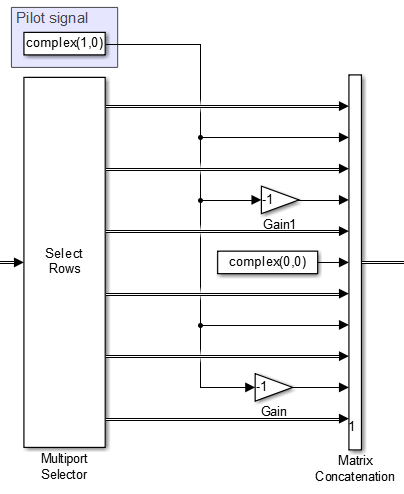
\includegraphics[width=7cm]{images/TX1.png}
\caption{OFDM transmitter first part that deals with the addressing of each subcarrier content. Source: own.}
\label{fig:ofdm:1} 
\end{center}
\end{figure}

It is important to say that the 4 pilot signals alternate between 1 and -1 and the DC subcarrier is modulated by 0. Both of this values are generated over a sample time of $8 \mu s$.

The second part of the transmitter can be seen in the figure \ref{fig:ofdm:2}. The first two blocks consists of a \textbf{Pad} block and a \textbf{Selector}. The pad block with \textbf{pad value} of 0 performs a zero pad to ensure its output to be of size 64 (equals to the size of the IFFT). Since the values are padded at the end of the sequence, the selector block will adjust the indexing with a indexing vector that takes the samples from 27 to 64 and put at the begin and the samples 1 to 26 are put at the end ($[27:64, 1:26]$).

\begin{figure}[h]
\begin{center}
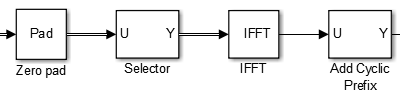
\includegraphics[width=8cm]{images/TX2.png}
\caption{OFDM transmitter second part that deals with the zero padding for guard bands, IFFT and cyclic prefix. Source: own.}
\label{fig:ofdm:2} 
\end{center}
\end{figure}

After configuring the zero padding, the \textbf{IFFT} is performed. Since the property of conjugate symmetry was not achieved, the output sequence is of type complex, but since the transmission will not have any additional modulation step this does not configure a problem. After the IFFT the \textbf{cyclic prefix}is inserted with the use of \textbf{selector} block that takes the $C=16$ last samples of the IFFT output and put them at the begin, e.g. since the cyclic prefix size is 16 and IFFT length is 64 the samples from 49 to 64 are repeated at the beginning of the block and the samples 1 to 64 are maintained at the end. 

This results in a OFDM symbol with a block of samples of size 80. Since the symbol time was previously set to $8\mu s$, perform the division $80/8 \mu$ results in a total occupied bandpass bandwidth of $10 MHz$ for the OFDM signal (the baseband bandwidth is half the value, i.e. $5 MHz$). This marks the end of the transmitter description.

\subsubsection{Channel}

In the standard OFDM transceiver after the transmitter block there is immediately the channel. The chosen channel was an \textbf{AWGN channel} with a homonymous block. The configuration of this block in very critical, so the output spectrum and, therefore the bit error rate can be measured as expected. The $E_bN_0$ value represents the normalized signal-to-noise-ratio and can be chosen as the designers wish (a higher $E_bN_0$ means a better signal quality and effective detection). THe parameter \textbf{number of bits per symbol} was set to the frame size $F_r = 192$ bits, once the OFDM symbol holds the entire frame. The \textbf{symbol period} was also set to match the sample time inside the transmitter, i.e. $8\mu s$. 

\begin{figure}[h]
\begin{center}
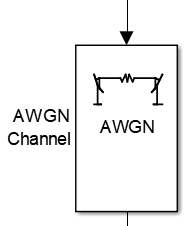
\includegraphics[width=3cm]{images/block4.png}
\caption{AWGN channel. Source: own.}
\label{fig:block4} 
\end{center}
\end{figure}

In the simulation a spectrum analyzer can be set in the output of the channel block so it tracks the OFDM signal spectrum.

\subsubsection{OFDM receiver}

The receiver objective is to undo all the changes that the transmitter performed in the primordial M-QAM symbols. To simplify the overall diagram a subsystem was used to hold all the receiver blocks. This subsystem is named OFDM receiver and can be seen in figure \ref{fig:block5}.


\begin{figure}[h]
\begin{center}
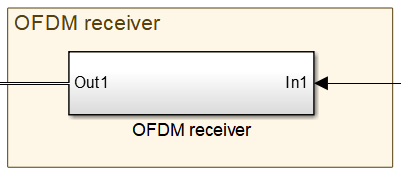
\includegraphics[width=5cm]{images/block5.png}
\caption{Higher layer from the OFDM receiver whose input comes from the channel and outputs the original M-QAM symbols. Source: own.}
\label{fig:block5} 
\end{center}
\end{figure}

Inside the subsystem there is the block chain of figure \ref{fig:ofdm:3}. Compared to the transmitter, the receiver is much simpler.

\begin{figure}[h]
\begin{center}
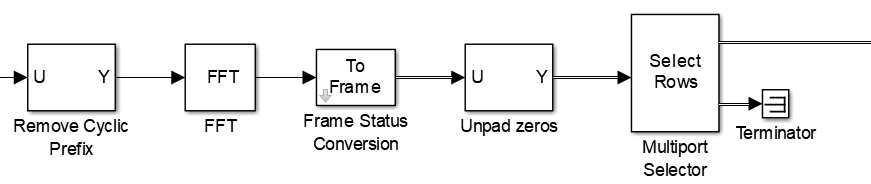
\includegraphics[width=8.5cm]{images/RX1.png}
\caption{OFDM receiver block chain. Source: own.}
\label{fig:ofdm:3} 
\end{center}
\end{figure}

The first block is a \textbf{remove cyclic prefix}, which is a \textbf{selector} that ignore the cyclic prefix inserted before. Since its size is $C=16$ samples, the first 16 samples are ignored, once those represent the cyclic prefix. The vector index of the selector ranges from 17 to 80. 

The output sequence has a resulting size of 64 samples whose pass through a \textbf{FFT} block of same size. Since the FFT removed the subcarriers influence the symbols can be manipulated freely.

The following block is a \textbf{frame status conversion} that will re-pack the symbols in a \textbf{frame-based} output. The next block is a \textbf{selector} to unpad the zeros added before, but first it need to rearrange the sequence with the following index vector: samples from 39 to 64 at the beginning and samples 1 to 27 at the end. 

Following the last \textbf{multiport selector} is used to extract the data symbols and the pilot symbols. The pilot symbols consisting of the samples 6, 20, 34 and 48 are thrown in a \textbf{terminator} block, since in this application they have no use. The remaining 48 samples are the data symbols (1 to 5, 7 to 19, 21 to 26, 28 to 33, 35 to 47 and 49 to 53) and they are thrown in the output of the subsystem direct to the M-QAM demodulator.

\subsubsection{Demodulate M-QAM symbols into bit frame}

The last section of blocks will demodulate the 48 16-QAM symbols into the original bit frame of 192 bits. The gain will \textbf{denormalize} the symbols multiplying by $\sqrt{M} = \sqrt{16}$ and the block \textbf{rectangular QAM demodulator baseband} will ensure that all modification made by its counterpart is undone.

\begin{figure}[h]
\begin{center}
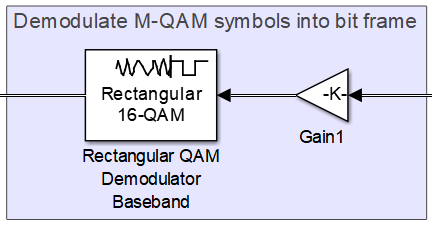
\includegraphics[width=5cm]{images/block6.png}
\caption{Rectangular QAM demodulator in baseband preceded by a positive  gain of which outputs to the target application or a error rate calculator. Source: own.}
\label{fig:block6} 
\end{center}
\end{figure}

This marks the end of the standard OFDM transceiver. 

\subsection{FIR filter design}

The design of the FIR filter for the f-OFDM signal will consist in the window function method and with the help of the Simulink block \texttt{fdatool}. The parameters for the f-OFDM signal are as shown in table \ref{table:1} adapted from \cite{cheng2016filtered} and the filter design will depend on its parameters. 

\begin{table}[H]
\centering
\caption{Comparison between datasheet and simulation result for insertion power gain at  $V_{cc} = 3V$ and $I_{cc} = 6mA$,}
\label{table:1}
\begin{tabular}{|c|c|c|}
\hline
\textbf{}                & \multicolumn{2}{c|}{\textbf{Insertion power gain $|s_{21}|^2$ (dB)}} \\ \hline
\textbf{Frequency (MHz)} & \textbf{Datasheet}               & \textbf{Simulation}               \\ \hline
100                      & 25                               & 24.964                            \\ \hline
150                      & 24.5                             & 24.765                            \\ \hline
450                      & 22.5                             & 22.511                            \\ \hline
900                      & 18.5                             & 18.753                            \\ \hline
1500                     & 14.5                             & 14.939                            \\ \hline
1900                     & 12.5                             & 12.939                            \\ \hline
2400                     & 10.5                             & 10.845                            \\ \hline
3500                     & 7                                & 7.054                             \\ \hline
\end{tabular}
\end{table}

The window function chosen for the filter was the Blackman-Harris window. The choice is justified by previous analysis of the frequency response of couple window functions. The analysis was made based in Wen (2009) \cite{wen2009hanning}.

The figure \ref{fig:win} is directly extracted from \cite{wen2009hanning} since it compares the magnitude response of 4 different windows of interest: Hamming, Hanning, Blackman and Blackman-Harris.


\begin{figure}[h]
\begin{center}
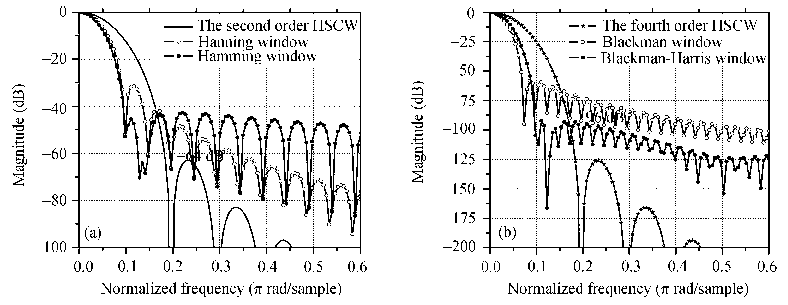
\includegraphics[width=8.5cm]{images/hbh.png}
\caption{Magnitude frequency response of various windows function. Source: Wen (2009) \cite{wen2009hanning}.}
\label{fig:win} 
\end{center}
\end{figure}

First comparing the Hamming and Hanning window between themselves, we can observe that the main lobe in each case resembles in terms of bandwidth occupied and amplitude. In terms of side lobes, the low frequency ones in the Hanning window have more significant amplitude, but decay firmly in high frequencies. Despite the high frequency side lobes for the Hamming frequency does not have a rapidly decay in amplitude, the value is reasonable and at low frequencies the side lobes are less influential than the Hanning window. 

Now comparing the Blackman and Blackman-Harris windows we observe that the latter has a higher pass band and the side lobes have low amplitude meaning a higher attenuation. Both have a passband lower than the Hanning and Hamming window and they promote a stronger attenuation in the rejection band.

So the Blackman-Harris window was chosen based primarily in its high attenuation characteristics in the rejection band. Also the use of Blackman-Harris window with a lower pass band compared to the Hamming or Hanning window is justified since the OFDM signal has guard bands. In this application we have 11 additional subcarriers uniformly distributed in each extremity of the signal spectrum. Since the carrier spacing is circa 125 kHz and 5 subcarriers from the guard band results in bandwidth of approximately 625 kHz in the worst scenario, the filter cutoff frequency can be set to a value higher than the subtraction between the 5 MHz of OFDM baseband bandwidth (that relates to a minimum sampling rate of 10 MHz) and the 625 kHz of single sided guard bands, resulting in a minimum cutoff frequency of 4.375 MHz. Therefore the filter cutoff frequency was defined as 4.2 MHz as a metric to compensate the low order of the filter. Further equalization could be implemented in the receiver to adjust the filter and channel distortion in the pass band.


\begin{comment}
After defining the window function, the next step in the filter design is to determine the cutoff frequency and its order. Since the sampling frequency was set to equal the bandpass bandwidth of the f-OFDM signal, which is 10 MHz, the maximum cutoff frequency must be less that half the sampling rate, therefore $< 5MHz$. Since it was reserved some guard bands, it does not configure major problems to filter out some of these. So the cutoff frequency was defined to be $4.5MHz$.
\end{comment}

Regarding the order of the filter it was chosen to have 96 coefficients. Once the transmitter and receiver filter are equal \cite{al2020improving}, this value denotes the overall delay in the transmission/reception chain. So the total delay provided by both filters combined is 192 samples, which is equivalent to the frame size. 

Also the low order was carefully chosen to not provoke a high forward and backward tail in the time response, since a higher order would require a even larger cyclic prefix, that would result in a high CP overhead \cite{zhang2015filtered}. 

The resulting magnitude response of the designed filter is represented in the figure \ref{fig:filter}. The response of the filter show little ripple in the pass band, ensuring a good flat response. In terms of rejection band, the side lobes are nearly nonexistent and does not present any major problem. Since the filter has a high order the cutoff frequency was respected with little distortion in the transition band.



\begin{figure}[h]
\begin{center}
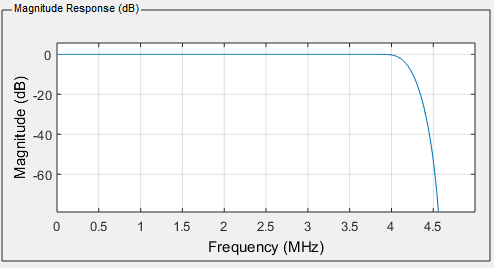
\includegraphics[width=8.5cm]{images/filter.png}
\caption{Magnitude response of the designed filter. Source: own.}
\label{fig:filter} 
\end{center}
\end{figure}

As a quick summary to the filter design, now we have:
\begin{itemize}
    \item Window function: Blackman-Harris;
    \item Sampling frequency: 10 MHz;
    \item Cutoff frequency: 4.2 MHz;
    \item Order: 96;
\end{itemize}

\subsection{Adding the filter to the transceiver}

Once the filter is designed with the help of the \texttt{fdatool}, we have to add it in the OFDM transmitter output and before the OFDM receiver input. 

In the transmission the filter will shape de OFDM signal reducing the side lobes bands and providing a waveforms that occupies a more restrict bandwidth. At the receiver the filter will undo the shaping made by it before and will return the OFDM signal as intended in the OFDM transmitter.
\section{Resultados e discussão}

Para encontrar todos os resultados necessários para comprovar a teoria, a prática foi dividida em algumas etapas, sendo elas:


\begin{itemize}

    \item Inicialmente foram montados os circuitos da figura \ref{ckt:1} e \ref{ckt:2};
    
    \item Para cada um dos circuitos foi utilizada uma senoide de 5V de pico (10V de pico-a-pico) e frequência variável na entrada, de forma que: $V_i(t) = 5sen(2\pi f t)$, para traçar a função de transferência de módulo e de fase para cada um dos circuitos;
    
    \item Com a mesma senoide do item anterior a frequência foi variada para encontrar a exata frequência de corte de cada filtro.
\end{itemize}

Para medir a frequência de corte de cada circuito os critérios de ganho e de fase foram utilizados, de forma que a frequência de corte ocorre na curva de Bode de ganho quando esta possui uma queda de 3dB. O critério de fase diverge para o filtro de 1ª ordem e o filtro de 2ª ordem, sendo que neste a frequência de corte ocorre em -90° e naquele ocorre em -45º na curva de Bode de fase.

Considerando o filtro passa-baixa de 1ª ordem, a frequência da tensão de entrada foi variada de 1Hz a 20kHz, permitindo obter os dados da tabela \ref{table:1}. Com esses dados foi possível montar as curvas de Bode da figura \ref{graph:1}. 

\begin{figure}[H]
\begin{center}
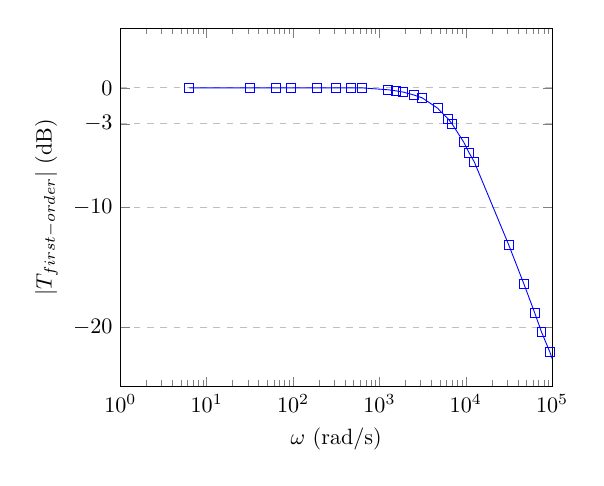
\begin{tikzpicture} [scale=0.8]
\begin{semilogxaxis}[
    title={},
    xlabel={$\omega$ (rad/s)},
    ylabel={$|T_{first-order}|$ (dB)},
    xmin=1, xmax=100000,
    ymin=-25, ymax=5,
    xtick={1,10,100,1000,10000,100000,1000000},
    ytick={0, -3, -10, -20},
    legend pos=north west,
    ymajorgrids=true,
    grid style=dashed,
]
\addplot[
    color=blue,
    mark=square,
    ]
    coordinates {
    (6.28,0)
    (31.42,0)
    (62.83,0)
    (94.25,0)
    (188.5,0)
    (314.16,0)
    (471.24,0)
    (628.32,0)
    (1256.64,-0.156)
    (1570.80,-0.253)
    (1884.96,-0.351)
    (2513.27,-0.596)
    (3141.59,-0.839)
    (4712.39,-1.694)
    (6283.19,-2.615)
    (6945.43,-3.012)
    (9424.78,-4.510)
    (10995.57,-5.465)
    (12566.37,-6.196)
    (31415.93,-13.120)
    (47123.89,-16.393)
    (62831.85,-18.808)
    (75398.22,-20.419)
    (94247.78,-22.099)
    (113097.34,-23.703)
    (125663.71,-24.324)
    };
\end{semilogxaxis}
\end{tikzpicture}
\hspace{1cm}
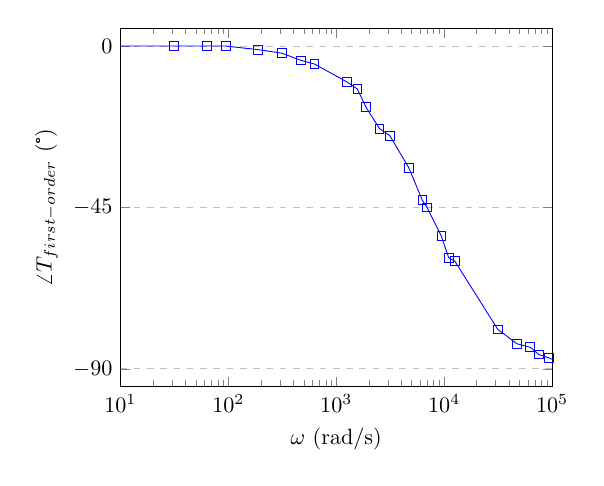
\begin{tikzpicture} [scale=0.8]
\begin{semilogxaxis}[
    title={},
    xlabel={$\omega$ (rad/s)},
    ylabel={$\angle T_{first-order}$ (°)},
    xmin=10, xmax=100000,
    ymin=-95, ymax=5,
    xtick={10,100,1000,10000,100000,1000000},
    ytick={0, -45, -90},
    legend pos=north west,
    ymajorgrids=true,
    grid style=dashed,
]
\addplot[
    color=blue,
    mark=square,
    ]
    coordinates {
    (6.28,0)
    (31.42,0)
    (62.83,0)
    (94.25,0)
    (188.5,-1)
    (314.16,-2)
    (471.24,-4)
    (628.32,-5)
    (1256.64,-10)
    (1570.80,-12)
    (1884.96,-17)
    (2513.27,-23)
    (3141.59,-25)
    (4712.39,-34)
    (6283.19,-43)
    (6945.43,-45)
    (9424.78,-53)
    (10995.57,-59)
    (12566.37,-60)
    (31415.93,-79)
    (47123.89,-83)
    (62831.85,-84)
    (75398.22,-86)
    (94247.78,-87)
    (113097.34,-88)
    (125663.71,-89)
    };
\end{semilogxaxis}
\end{tikzpicture}
\end{center}
\caption{Curvas de bode com os resultados práticos da função de transferência do filtro passa-baixas de 1ª ordem.}
\label{graph:1} 
\end{figure}

No filtro passa-baixa de 1ª ordem esperava-se que para uma tensão de entrada de 10V de pico-a-pico, a saída fosse de 7.07 V de pico-a-pico e que a defasagem entre a forma de onda de tensão da entrada e da saída fosse de -45°. Isso foi perfeitamente obtido na prática, da forma como foi encontrada na tabela e cujas formas de onda podem ser observadas na figura \ref{fo1}.

\begin{figure}[H] 
\centering
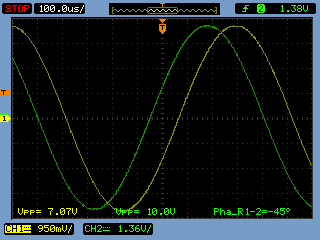
\includegraphics[width=7cm]{images/f0_1.png}
\caption{Formas de onda obtidas no osciloscópio para o filtro passa-baixa de 1ª ordem na frequência de corte, sendo a saída no CH1 e a entrada no CH2.}
\label{fo1} 
\end{figure}

A frequência de corte obtida na prática foi de 1105.4Hz, uma vez que a esperada era de 1061Hz, o erro relacionado à frequência é de 4.01\%.

A partir dos dados da tabela \ref{table:1}, se escolher o ganho para a frequência de 2kHz (-6.196 dB) e o ganho uma década depois, ou seja, em 20kHz (-24.324 dB), observa-se um queda de 18.128 dB, um valor bem próximo do esperado pela curva teórica, que é uma atenuação de 20 dB por década, com um erro de 9.36\%. Ao conferir as curvas de Bode da figura \ref{graph:1}, observa-se uma boa concordância com as curvas da figura \ref{fig:3} obtidas no MATLAB.

Para o  filtro passa-baixa de 2ª ordem, a frequência da tensão de entrada também foi variada de 1Hz a 20kHz, permitindo obter os dados da tabela \ref{table:2}. Com esses dados foi possível montar as curvas de Bode da figura \ref{graph:2}. 

\begin{figure}[H]
\begin{center}
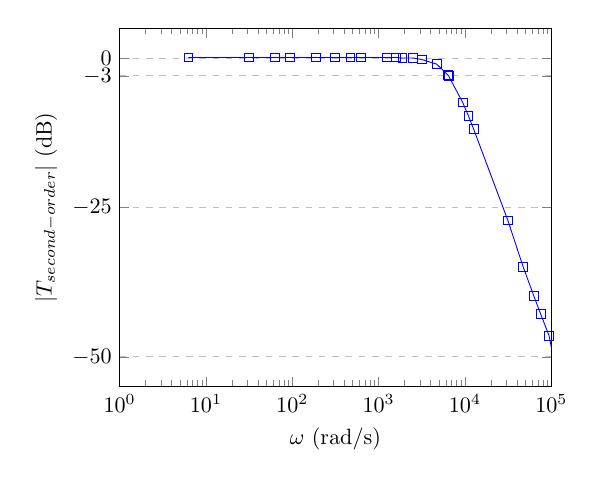
\begin{tikzpicture} [scale=0.8]
\begin{semilogxaxis}[
    title={},
    xlabel={$\omega$ (rad/s)},
    ylabel={$|T_{second-order}|$ (dB)},
    xmin=1, xmax=100000,
    ymin=-55, ymax=5,
    xtick={1,10,100,1000,10000,100000,1000000},
    ytick={0, -3, -25, -50},
    legend pos=north west,
    ymajorgrids=true,
    grid style=dashed,
]
\addplot[
    color=blue,
    mark=square,
    ]
    coordinates {
    (6.28,0.086)
    (31.42,0.086)
    (62.83,0.086)
    (94.25,0.086)
    (188.5,0.086)
    (314.16,0.086)
    (471.24,0.086)
    (628.32,0.086)
    (1256.64,0.086)
    (1570.80,0.086)
    (1884.96,0)
    (2513.27,0)
    (3141.59,-0.244)
    (4712.39,-1.031)
    (6283.19,-2.796)
    (6477.96,-3.012)
    (9424.78,-7.447)
    (10995.57,-9.710)
    (12566.37,-11.843)
    (31415.93,-27.171)
    (47123.89,-34.895)
    (62831.85,-39.830)
    (75398.22,-42.844)
    (94247.78,-46.462)
    (113097.34,-52.197)
    (125663.71,-54.420)
    };
\end{semilogxaxis}
\end{tikzpicture}
\hspace{1cm}
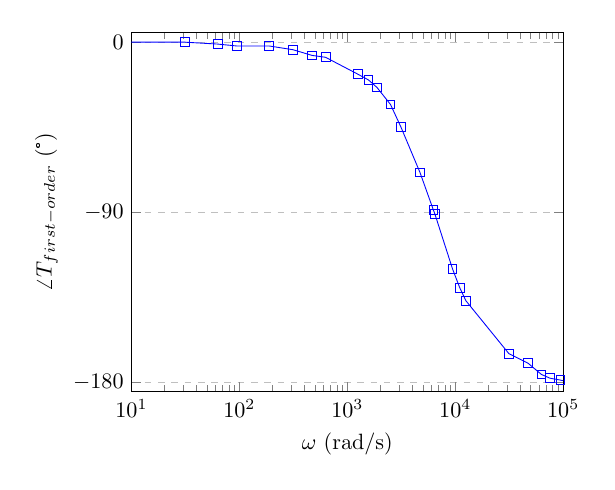
\begin{tikzpicture} [scale=0.8]
\begin{semilogxaxis}[
    title={},
    xlabel={$\omega$ (rad/s)},
    ylabel={$\angle T_{first-order}$ (°)},
    xmin=10, xmax=100000,
    ymin=-185, ymax=5,
    xtick={10,100,1000,10000,100000,1000000},
    ytick={0, -90, -180},
    legend pos=north west,
    ymajorgrids=true,
    grid style=dashed,
]
\addplot[
    color=blue,
    mark=square,
    ]
    coordinates {
    (6.28,0)
    (31.42,0)
    (62.83,-1)
    (94.25,-2)
    (188.5,-2)
    (314.16,-4)
    (471.24,-7)
    (628.32,-8)
    (1256.64,-17)
    (1570.80,-20)
    (1884.96,-24)
    (2513.27,-33)
    (3141.59,-45)
    (4712.39,-69)
    (6283.19,-89)
    (6477.96,-91)
    (9424.78,-120)
    (10995.57,-130)
    (12566.37,-137)
    (31415.93,-165)
    (47123.89,-170)
    (62831.85,-176)
    (75398.22,-178)
    (94247.78,-179)
    (113097.34,-180)
    (125663.71,-180)
    };
\end{semilogxaxis}
\end{tikzpicture}
\end{center}
\caption{Curvas de bode com os resultados práticos da função de transferência do filtro passa-baixas de 2ª ordem}
\label{graph:2} 
\end{figure}

No filtro passa-baixa de 2ª ordem, esperava-se que para uma tensão de entrada de 10V de pico-a-pico, a saída fosse de 7.07 V de pico-a-pico e que a defasagem entre a forma de onda de tensão da entrada e da saída fosse de -90°. Isso foi quase que perfeitamente obtido na prática, da forma como foi encontrada na tabela e cujas formas de onda podem ser observadas na figura \ref{fo2}, com uma defasagem de -91° ao invés de 90°, com um erro de 1.09\%.

\begin{figure}[H] 
\centering
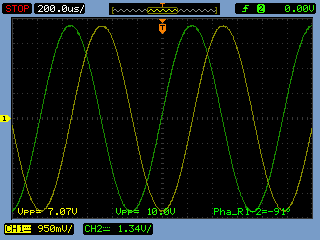
\includegraphics[width=7cm]{images/f0_2.png}
\caption{Formas de onda obtidas no osciloscópio para o filtro passa-baixa de 2ª ordem na frequência de corte, sendo a saída no CH1 e a entrada no CH2.}
\label{fo2} 
\end{figure}

A frequência de corte obtida na prática foi de 1031Hz, uma vez que a esperada era de 967.51Hz, o erro relacionado à frequência é de 6.15\%.

A partir dos dados da tabela \ref{table:1}, se escolher o ganho para a frequência de 2kHz (-11.843 dB) e o ganho uma década depois, ou seja, em 20kHz (-54.420 dB), observa-se um queda de 42.577 dB, um valor bem próximo do esperado pela curva teórica, que é uma atenuação de 40 dB por década, com um erro de 6.05\%. Ao conferir as curvas de Bode da figura \ref{graph:2}, observa-se uma boa concordância com as curvas da figura \ref{fig:4} obtidas no MATLAB.

Uma medida importante do filtro de 2ª ordem é o seu fator de qualidade (Q). Reconhecendo a forma geral da função de transferência de um filtro de segunda ordem na equação \ref{q1} e os seus polos na equação \ref{q2}, observa-se que a um valor alto de Q permite que a distância dos polos até o eixo $j\omega$ diminua, tornando assim o filtro mais seletivo.

\begin{equation} \label{q1}
    T(s) = \frac{a_2s^2+a_1s+a_0}{s^2+(\omega/Q)s+\omega^2}
\end{equation}

\begin{equation} \label{q2}
    p_1, p_2 = -\frac{\omega}{2Q}\pm j\omega\sqrt{1-(1/4Q)^2}
\end{equation}

Para o caso do filtro de 2ª ordem implementado na prática, o valor de Q é 0.709, que é um valor próximo de 0.707, cuja resposta obtida para esse fator de qualidade é chamada Butterworth, ou a resposta mais achatada e que foi constatada na prática. Na figura \ref{Q} observa-se que ao diminuir o fator Q da função de transferência do filtro passa-baixa de segunda ordem o filtro se torna menos seletivo e, de acordo com que Q aumenta, a seletividade aumenta, porém a resposta apresenta picos de ressonância na frequência de corte. 

\begin{figure}[H] 
\centering
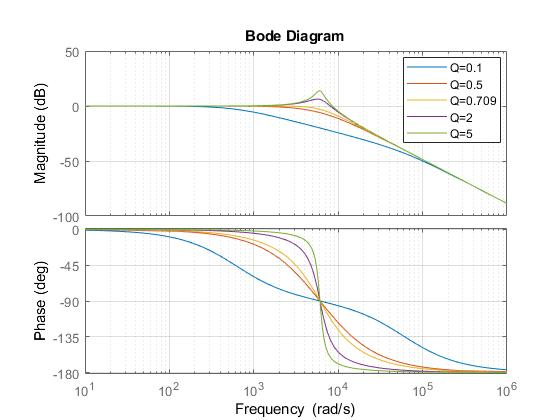
\includegraphics[width=14cm]{images/BodeQ.jpg}
\caption{Ensaios para valores variáveis de Q na função de transferência do filtro passa-baixas de 2ª ordem.}
\label{Q} 
\end{figure}

Por fim a figura \ref{graph:3} mostra a comparação direta das curvas de Bode do filtro passa-baixas de 1ª e 2ª ordem, mostrando que de fato o filtro de 2ª ordem possui uma maior seletividade representada na capacidade de atenuar frequências acima da de corte com um fator 40dB por década, ao passo que o filtro de 1ª ordem só atenua 20dB por década. Porém esta conclusão não tira o mérito do filtro de 1ª ordem, pois ele ainda se apresenta uma alternativa um pouco mais barata ao filtro de 2ª ordem.

\begin{figure}[H]
\begin{center}
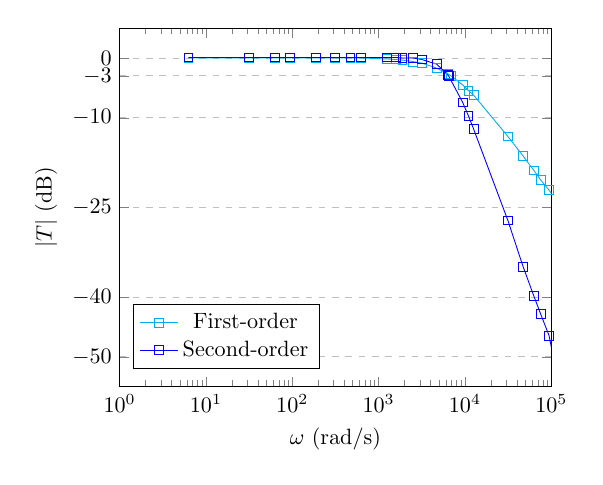
\begin{tikzpicture} [scale=0.8]
\begin{semilogxaxis}[
    title={},
    xlabel={$\omega$ (rad/s)},
    ylabel={$|T|$ (dB)},
    xmin=1, xmax=100000,
    ymin=-55, ymax=5,
    xtick={1,10,100,1000,10000,100000,1000000},
    ytick={0, -3, -10, -25, -40, -50},
    legend pos=north west,
    ymajorgrids=true,
    grid style=dashed,
    legend style={at={(0.03,0.05)},anchor=south west},
]
\addplot[
    color=cyan,
    mark=square,
    ]
    coordinates {
    (6.28,0)
    (31.42,0)
    (62.83,0)
    (94.25,0)
    (188.5,0)
    (314.16,0)
    (471.24,0)
    (628.32,0)
    (1256.64,-0.156)
    (1570.80,-0.253)
    (1884.96,-0.351)
    (2513.27,-0.596)
    (3141.59,-0.839)
    (4712.39,-1.694)
    (6283.19,-2.615)
    (6945.43,-3.012)
    (9424.78,-4.510)
    (10995.57,-5.465)
    (12566.37,-6.196)
    (31415.93,-13.120)
    (47123.89,-16.393)
    (62831.85,-18.808)
    (75398.22,-20.419)
    (94247.78,-22.099)
    (113097.34,-23.703)
    (125663.71,-24.324)
    }; \addlegendentry{First-order}
\addplot[
    color=blue,
    mark=square,
    ]
    coordinates {
    (6.28,0.086)
    (31.42,0.086)
    (62.83,0.086)
    (94.25,0.086)
    (188.5,0.086)
    (314.16,0.086)
    (471.24,0.086)
    (628.32,0.086)
    (1256.64,0.086)
    (1570.80,0.086)
    (1884.96,0)
    (2513.27,0)
    (3141.59,-0.244)
    (4712.39,-1.031)
    (6283.19,-2.796)
    (6477.96,-3.012)
    (9424.78,-7.447)
    (10995.57,-9.710)
    (12566.37,-11.843)
    (31415.93,-27.171)
    (47123.89,-34.895)
    (62831.85,-39.830)
    (75398.22,-42.844)
    (94247.78,-46.462)
    (113097.34,-52.197)
    (125663.71,-54.420)
    }; \addlegendentry{Second-order}
\end{semilogxaxis}
\end{tikzpicture}
\hspace{1cm}
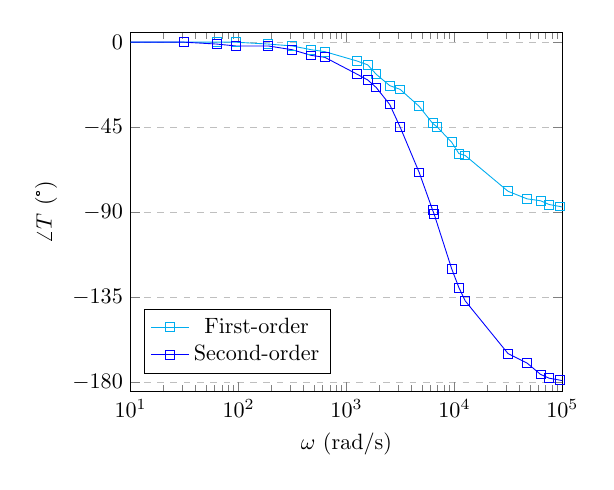
\begin{tikzpicture} [scale=0.8]
\begin{semilogxaxis}[
    title={},
    xlabel={$\omega$ (rad/s)},
    ylabel={$\angle T$ (°)},
    xmin=10, xmax=100000,
    ymin=-185, ymax=5,
    xtick={10,100,1000,10000,100000,1000000},
    ytick={0, -45, -90, -135, -180},
    legend pos=north west,
    ymajorgrids=true,
    grid style=dashed,
    legend style={at={(0.03,0.05)},anchor=south west},
]
\addplot[
    color=cyan,
    mark=square,
    ]
    coordinates {
    (6.28,0)
    (31.42,0)
    (62.83,0)
    (94.25,0)
    (188.5,-1)
    (314.16,-2)
    (471.24,-4)
    (628.32,-5)
    (1256.64,-10)
    (1570.80,-12)
    (1884.96,-17)
    (2513.27,-23)
    (3141.59,-25)
    (4712.39,-34)
    (6283.19,-43)
    (6945.43,-45)
    (9424.78,-53)
    (10995.57,-59)
    (12566.37,-60)
    (31415.93,-79)
    (47123.89,-83)
    (62831.85,-84)
    (75398.22,-86)
    (94247.78,-87)
    (113097.34,-88)
    (125663.71,-89)
    }; \addlegendentry{First-order}
\addplot[
    color=blue,
    mark=square,
    ]
    coordinates {
    (6.28,0)
    (31.42,0)
    (62.83,-1)
    (94.25,-2)
    (188.5,-2)
    (314.16,-4)
    (471.24,-7)
    (628.32,-8)
    (1256.64,-17)
    (1570.80,-20)
    (1884.96,-24)
    (2513.27,-33)
    (3141.59,-45)
    (4712.39,-69)
    (6283.19,-89)
    (6477.96,-91)
    (9424.78,-120)
    (10995.57,-130)
    (12566.37,-137)
    (31415.93,-165)
    (47123.89,-170)
    (62831.85,-176)
    (75398.22,-178)
    (94247.78,-179)
    (113097.34,-180)
    (125663.71,-180)
    }; \addlegendentry{Second-order}
\end{semilogxaxis}
\end{tikzpicture}
\end{center}
\caption{Comparação entre as funções de transferência de cada filtro.}
\label{graph:3} 
\end{figure}


%\newpage
\section{Conclusões}

O controle digital por computador se mostrou uma boa alternativa ao controle analógico tradicional, pois ele permite a facilidade de reprojeto e um ambiente com condições externas controladas, evitando ter que se preocupar com fatores limitantes do ambiente ou de tolerância de componentes. Porém, como a representação digital é apenas uma aproximação da representação analógica, a velocidade no processamento dos dados será um barreira limitante, pois ela dita a precisão do modelo. Entretanto, ao obedecer o teorema da amostragem e conhecimento prévio do hardware no qual o controlador será implementado, as barreiras limitantes diminuem, permitindo a expansão das técnicas de controle tradicionais para novos horizontes de aplicações.
\pagebreak
\begin{thebibliography}{99}
\bibitem{b1} de Lauro Castrucci, Plínio Benedicto, e Anselmo Bittar. Controle automático. Grupo Gen-LTC, 2000.
\bibitem{b2} Kuo, Benjamin C., e Farid Golnaraghi. Automatic control systems. Vol. 9. Englewood Cliffs, NJ: Prentice-Hall, 1995.
\bibitem{b3} Introduction to Control Systems in Scilab. Disponível em: \url{http://www.openeering.com/}.
\bibitem{b4} Ogata, Katsuhiko. Modern control engineering. Upper Saddle River, NJ: Prentice Hall, 2009.
\bibitem{b5} Sedra, Adel S., et al. Microelectronic circuits. Oxford University Press, 2016.
\end{thebibliography}

\pagebreak




\addtolength{\textheight}{-12cm}  

\begin{comment}
\section*{APPENDIX}

Appendixes should appear before the acknowledgment.

\section*{ACKNOWLEDGMENT}

The preferred spelling of the word ``acknowledgment'' in America is without an ``e'' after the ``g''. Avoid the stilted expression, ``One of us (R. B. G.) thanks . . .''  Instead, try ``R. B. G. thanks''. Put sponsor acknowledgments in the unnumbered footnote on the first page.



%%%%%%%%%%%%%%%%%%%%%%%%%%%%%%%%%%%%%%%%%%%%%%%%%%%%%%%%%%%%%%%%%%%%%%%%%%%%%%%%

References are important to the reader; therefore, each citation must be complete and correct. If at all possible, references should be commonly available publications.

\end{comment}






\end{document}
